% Options for packages loaded elsewhere
\PassOptionsToPackage{unicode}{hyperref}
\PassOptionsToPackage{hyphens}{url}
%
\documentclass[
  a4paper,
]{article}
\usepackage{amsmath,amssymb}
\usepackage{setspace}
\usepackage{iftex}
\ifPDFTeX
  \usepackage[T1]{fontenc}
  \usepackage[utf8]{inputenc}
  \usepackage{textcomp} % provide euro and other symbols
\else % if luatex or xetex
  \usepackage{unicode-math} % this also loads fontspec
  \defaultfontfeatures{Scale=MatchLowercase}
  \defaultfontfeatures[\rmfamily]{Ligatures=TeX,Scale=1}
\fi
\usepackage{lmodern}
\ifPDFTeX\else
  % xetex/luatex font selection
\fi
% Use upquote if available, for straight quotes in verbatim environments
\IfFileExists{upquote.sty}{\usepackage{upquote}}{}
\IfFileExists{microtype.sty}{% use microtype if available
  \usepackage[]{microtype}
  \UseMicrotypeSet[protrusion]{basicmath} % disable protrusion for tt fonts
}{}
\makeatletter
\@ifundefined{KOMAClassName}{% if non-KOMA class
  \IfFileExists{parskip.sty}{%
    \usepackage{parskip}
  }{% else
    \setlength{\parindent}{0pt}
    \setlength{\parskip}{6pt plus 2pt minus 1pt}}
}{% if KOMA class
  \KOMAoptions{parskip=half}}
\makeatother
\usepackage{xcolor}
\usepackage[margin=1in]{geometry}
\usepackage{color}
\usepackage{fancyvrb}
\newcommand{\VerbBar}{|}
\newcommand{\VERB}{\Verb[commandchars=\\\{\}]}
\DefineVerbatimEnvironment{Highlighting}{Verbatim}{commandchars=\\\{\}}
% Add ',fontsize=\small' for more characters per line
\usepackage{framed}
\definecolor{shadecolor}{RGB}{248,248,248}
\newenvironment{Shaded}{\begin{snugshade}}{\end{snugshade}}
\newcommand{\AlertTok}[1]{\textcolor[rgb]{0.94,0.16,0.16}{#1}}
\newcommand{\AnnotationTok}[1]{\textcolor[rgb]{0.56,0.35,0.01}{\textbf{\textit{#1}}}}
\newcommand{\AttributeTok}[1]{\textcolor[rgb]{0.13,0.29,0.53}{#1}}
\newcommand{\BaseNTok}[1]{\textcolor[rgb]{0.00,0.00,0.81}{#1}}
\newcommand{\BuiltInTok}[1]{#1}
\newcommand{\CharTok}[1]{\textcolor[rgb]{0.31,0.60,0.02}{#1}}
\newcommand{\CommentTok}[1]{\textcolor[rgb]{0.56,0.35,0.01}{\textit{#1}}}
\newcommand{\CommentVarTok}[1]{\textcolor[rgb]{0.56,0.35,0.01}{\textbf{\textit{#1}}}}
\newcommand{\ConstantTok}[1]{\textcolor[rgb]{0.56,0.35,0.01}{#1}}
\newcommand{\ControlFlowTok}[1]{\textcolor[rgb]{0.13,0.29,0.53}{\textbf{#1}}}
\newcommand{\DataTypeTok}[1]{\textcolor[rgb]{0.13,0.29,0.53}{#1}}
\newcommand{\DecValTok}[1]{\textcolor[rgb]{0.00,0.00,0.81}{#1}}
\newcommand{\DocumentationTok}[1]{\textcolor[rgb]{0.56,0.35,0.01}{\textbf{\textit{#1}}}}
\newcommand{\ErrorTok}[1]{\textcolor[rgb]{0.64,0.00,0.00}{\textbf{#1}}}
\newcommand{\ExtensionTok}[1]{#1}
\newcommand{\FloatTok}[1]{\textcolor[rgb]{0.00,0.00,0.81}{#1}}
\newcommand{\FunctionTok}[1]{\textcolor[rgb]{0.13,0.29,0.53}{\textbf{#1}}}
\newcommand{\ImportTok}[1]{#1}
\newcommand{\InformationTok}[1]{\textcolor[rgb]{0.56,0.35,0.01}{\textbf{\textit{#1}}}}
\newcommand{\KeywordTok}[1]{\textcolor[rgb]{0.13,0.29,0.53}{\textbf{#1}}}
\newcommand{\NormalTok}[1]{#1}
\newcommand{\OperatorTok}[1]{\textcolor[rgb]{0.81,0.36,0.00}{\textbf{#1}}}
\newcommand{\OtherTok}[1]{\textcolor[rgb]{0.56,0.35,0.01}{#1}}
\newcommand{\PreprocessorTok}[1]{\textcolor[rgb]{0.56,0.35,0.01}{\textit{#1}}}
\newcommand{\RegionMarkerTok}[1]{#1}
\newcommand{\SpecialCharTok}[1]{\textcolor[rgb]{0.81,0.36,0.00}{\textbf{#1}}}
\newcommand{\SpecialStringTok}[1]{\textcolor[rgb]{0.31,0.60,0.02}{#1}}
\newcommand{\StringTok}[1]{\textcolor[rgb]{0.31,0.60,0.02}{#1}}
\newcommand{\VariableTok}[1]{\textcolor[rgb]{0.00,0.00,0.00}{#1}}
\newcommand{\VerbatimStringTok}[1]{\textcolor[rgb]{0.31,0.60,0.02}{#1}}
\newcommand{\WarningTok}[1]{\textcolor[rgb]{0.56,0.35,0.01}{\textbf{\textit{#1}}}}
\usepackage{longtable,booktabs,array}
\usepackage{calc} % for calculating minipage widths
% Correct order of tables after \paragraph or \subparagraph
\usepackage{etoolbox}
\makeatletter
\patchcmd\longtable{\par}{\if@noskipsec\mbox{}\fi\par}{}{}
\makeatother
% Allow footnotes in longtable head/foot
\IfFileExists{footnotehyper.sty}{\usepackage{footnotehyper}}{\usepackage{footnote}}
\makesavenoteenv{longtable}
\usepackage{graphicx}
\makeatletter
\def\maxwidth{\ifdim\Gin@nat@width>\linewidth\linewidth\else\Gin@nat@width\fi}
\def\maxheight{\ifdim\Gin@nat@height>\textheight\textheight\else\Gin@nat@height\fi}
\makeatother
% Scale images if necessary, so that they will not overflow the page
% margins by default, and it is still possible to overwrite the defaults
% using explicit options in \includegraphics[width, height, ...]{}
\setkeys{Gin}{width=\maxwidth,height=\maxheight,keepaspectratio}
% Set default figure placement to htbp
\makeatletter
\def\fps@figure{htbp}
\makeatother
\setlength{\emergencystretch}{3em} % prevent overfull lines
\providecommand{\tightlist}{%
  \setlength{\itemsep}{0pt}\setlength{\parskip}{0pt}}
\setcounter{secnumdepth}{-\maxdimen} % remove section numbering
\ifLuaTeX
\usepackage[bidi=basic]{babel}
\else
\usepackage[bidi=default]{babel}
\fi
\babelprovide[main,import]{catalan}
% get rid of language-specific shorthands (see #6817):
\let\LanguageShortHands\languageshorthands
\def\languageshorthands#1{}
\ifLuaTeX
  \usepackage{selnolig}  % disable illegal ligatures
\fi
\usepackage{bookmark}
\IfFileExists{xurl.sty}{\usepackage{xurl}}{} % add URL line breaks if available
\urlstyle{same}
\hypersetup{
  pdftitle={U5. LUBUNTU. ESTRUCTURA},
  pdfauthor={@tofermos 2024},
  pdflang={ca-ES},
  hidelinks,
  pdfcreator={LaTeX via pandoc}}

\title{U5. LUBUNTU. ESTRUCTURA}
\author{@tofermos 2024}
\date{}

\begin{document}
\maketitle

{
\setcounter{tocdepth}{2}
\tableofcontents
}
\setstretch{1.5}
\newpage
\renewcommand\tablename{Tabla}

\section{1. El sistema operatiu GNU/Linux.
Característiques}\label{el-sistema-operatiu-gnulinux.-caracteruxedstiques}

\subsection{1.1 El sistema operatiu
GNU/Linux}\label{el-sistema-operatiu-gnulinux}

\begin{itemize}
\tightlist
\item
  \textbf{GNU/Linux} és un sistema operatiu lliure i de codi obert.
\item
  Basat en el nucli \textbf{Linux} i eines del projecte \textbf{GNU}.
\item
  Escalable: pot ser utilitzat en dispositius menuts o grans servidors.
\end{itemize}

\section{1.2 Distribucions}\label{distribucions}

Una \textbf{distribució} Linux (distro) és un sistema operatiu basat en
el nucli Linux que inclou programari específic, eines d'administració,
gestors de paquets i una configuració personalitzada. Cada distribució
s'adapta a necessitats concretes:ús general, educació, servidors,
sistemes lleugers\ldots{}

Exemples de distribucions:

\begin{longtable}[]{@{}ll@{}}
\toprule\noalign{}
\textbf{Distribució} & \textbf{Orientació} \\
\midrule\noalign{}
\endhead
\bottomrule\noalign{}
\endlastfoot
Ubuntu & Usuaris nous, suport comunitari. \\
Debian & Estable, per servidors. \\
Arch Linux & Personalitzable, usuaris experts. \\
Fedora & \\
Manjaro & \\
\end{longtable}

Als cicles de FP ens centrarem en \textbf{Ubuntu}

\subsection{1.4 Característiques
d'Ubuntu}\label{caracteruxedstiques-dubuntu}

\begin{itemize}
\tightlist
\item
  \textbf{Lliure i obert}: Es pot modificar i distribuir.
\item
  \textbf{Multiusuari}: Diversos usuaris alhora.
\item
  \textbf{Multitasca}: Execució de múltiples processos.
\item
  \textbf{Segur}: Model de permisos.
\item
  \textbf{Portabilitat}: Funciona en diferents plataformes.
\end{itemize}

\section{2. La Instal·lació de
Ubuntu}\label{la-installaciuxf3-de-ubuntu}

\subsection{2.1 Pasos}\label{pasos}

\begin{enumerate}
\def\labelenumi{\arabic{enumi}.}
\tightlist
\item
  Descarrega la imatge ISO des d'\href{https://ubuntu.com/}{ubuntu.com}.
\item
  Comprova que l'has descarregada bé ( codi HASH: \texttt{sha256sum},
  habitualment )
\item
  Grava-la en un PenDrive amb eines com \textbf{Ventoy} (o Rufus,
  Etcher).
\item
  Modifica el BootOrder de la UEFI per arrancar des del PenDrive.
\item
  Segueix el procés d'instal·lació: Partició SWAP (si en necessites),
  regióm idioma, fus horari, altres particions.
\item
  Canvia el BootOrder i incia sessió.
\end{enumerate}

\subsection{2.2 Versió d'Ubuntu}\label{versiuxf3-dubuntu}

Amb l'ordre:

\begin{Shaded}
\begin{Highlighting}[]
\ExtensionTok{lsb\_release} \AttributeTok{{-}a}
\end{Highlighting}
\end{Shaded}

o llegint el fitxer de configuració

\begin{Shaded}
\begin{Highlighting}[]
\FunctionTok{cat}\NormalTok{ /etc/os{-}release}
\end{Highlighting}
\end{Shaded}

Una vegada més veiem com en un fitxer de text pla es guarda informació
del sistema. En este cas:

\begin{itemize}
\tightlist
\item
  Nom del SO
\item
  Distribució
\item
  Versió
\end{itemize}

I el fitxer el manté una ordre: lsb\_release

\section{3 Estructura}\label{estructura}

\subsection{3.1 Nucli (Kernel)}\label{nucli-kernel}

\begin{itemize}
\tightlist
\item
  Gestió de recursos: memòria, CPU, dispositius.
\item
  Per veure la versió: \texttt{bash\ \ \ \ \ \ uname\ -r}
\item
  Exemple de resultat: \texttt{6.8.0-49-generic}.
\end{itemize}

\subsection{3.2 Shell}\label{shell}

\subsubsection{Definicio i tipus}\label{definicio-i-tipus}

\begin{itemize}
\tightlist
\item
  Interfície que permet interactuar amb el sistema amb les seues ordres.
\item
  Exemples: \textbf{bash}, \textbf{sh}, \textbf{dash}.
\end{itemize}

Els shells diponible sels tenim al fitxer /etc/shells

\begin{Shaded}
\begin{Highlighting}[]
\FunctionTok{cat}\NormalTok{ /etc/shells}
\end{Highlighting}
\end{Shaded}

Cada usuari té un assigant (ho podem vore a /etc/passwd) però es pot
canviar amb: chsh ( change shell)

\begin{Shaded}
\begin{Highlighting}[]
\FunctionTok{sudo}\NormalTok{ chsh }\AttributeTok{{-}s}\NormalTok{ /bin/bash tomas}
\end{Highlighting}
\end{Shaded}

El canvi es vorà immediatament en /etc/passwd però no s'aplicarà fins
que no reiniciem sessió amb l'usuari.

\subsubsection{Ordres}\label{ordres}

\begin{itemize}
\tightlist
\item
  Comandes bàsiques: \texttt{ls}, \texttt{cp}, \texttt{mv}.
\end{itemize}

\subsubsection{Utilitats}\label{utilitats}

\texttt{apt}, ǹet-tools\texttt{,}mdadm',

\subsubsection{Curiositats}\label{curiositats}

Podem instal·lar un emulador del shell més avançat de MS-Windows a
Ubuntu: el PowerShell.

\subsection{3.3 Entorn gràfic}\label{entorn-gruxe0fic}

\subsubsection{3.3.1 Entorn d'escriptori}\label{entorn-descriptori}

Un \textbf{entorn d'escriptori} és el conjunt d'elements gràfics que
defineixen la interfície visual del sistema operatiu. Inclou la gestió
de finestres, menús, barres d'eines, icones i aplicacions
predeterminades, com el gestor d'arxius o l'emulador de terminal.

CAda Distro en porta un per defecte que podem canviar i tindre un altre
o més d'un i triar en l'inici de sessió d'usuari.

\textbf{Exemples:} Gnome, KDE Plasma, Xfce, LXQt, Mate, Cinnamon.

\subsubsection{3.3.2 Gestor d'arxius}\label{gestor-darxius}

Un \textbf{gestor d'arxius} és una aplicació que permet navegar,
organitzar, copiar, moure i gestionar fitxers i carpetes del sistema. És
una peça essencial en qualsevol entorn d'escriptori.

Per defecte cada Entorn d'Escriptori en duu un però podem instal·lar i
desinstal·lar-ne, tindre'n més d'un\ldots{}

\textbf{Exemples:} Nautilus (Gnome), Dolphin (KDE Plasma), Thunar
(Xfce), PCManFM-Qt (LXQt).

\subsubsection{3.3.3 Emulador de terminal}\label{emulador-de-terminal}

Un \textbf{emulador de terminal} és una aplicació que proporciona accés
a la línia de comandes. Permet interactuar directament amb el sistema
operatiu, executar ordres, i gestionar processos i fitxers de manera
avançada.

Per defecte cada Entorn d'Escriptori en duu un però (igual que amb el
Gestor de Fitxers) podem instal·lar i desinstal·lar-ne, tindre'n més
d'un\ldots{}

\textbf{Exemples:} Gnome Terminal, Konsole (KDE), Xfce Terminal,
QTerminal (LXQt).

\begin{center}\rule{0.5\linewidth}{0.5pt}\end{center}

\section{\texorpdfstring{4 L'\emph{ecosistema} gràfic de
Linux}{4 L'ecosistema gràfic de Linux}}\label{lecosistema-gruxe0fic-de-linux}

\subsection{4.1 Quadre resum}\label{quadre-resum}

\begin{longtable}[]{@{}
  >{\raggedright\arraybackslash}p{(\columnwidth - 10\tabcolsep) * \real{0.1137}}
  >{\raggedright\arraybackslash}p{(\columnwidth - 10\tabcolsep) * \real{0.1185}}
  >{\raggedright\arraybackslash}p{(\columnwidth - 10\tabcolsep) * \real{0.2512}}
  >{\raggedright\arraybackslash}p{(\columnwidth - 10\tabcolsep) * \real{0.1517}}
  >{\raggedright\arraybackslash}p{(\columnwidth - 10\tabcolsep) * \real{0.1991}}
  >{\raggedright\arraybackslash}p{(\columnwidth - 10\tabcolsep) * \real{0.1659}}@{}}
\toprule\noalign{}
\begin{minipage}[b]{\linewidth}\raggedright
\textbf{Distribució}
\end{minipage} & \begin{minipage}[b]{\linewidth}\raggedright
\textbf{Entorn d'escriptori}
\end{minipage} & \begin{minipage}[b]{\linewidth}\raggedright
\textbf{Usos habituals}
\end{minipage} & \begin{minipage}[b]{\linewidth}\raggedright
\textbf{Paquet}
\end{minipage} & \begin{minipage}[b]{\linewidth}\raggedright
\textbf{Gestor d'arxius per defecte} (paquet)
\end{minipage} & \begin{minipage}[b]{\linewidth}\raggedright
\textbf{Emulador de terminal per defecte} (paquet)
\end{minipage} \\
\midrule\noalign{}
\endhead
\bottomrule\noalign{}
\endlastfoot
\textbf{Lubuntu} & \textbf{LXQt} & Perfecte per a equips molt antics o
amb pocs recursos. & \texttt{lubuntu-desktop} & \textbf{PCManFM-Qt
(\texttt{pcmanfm-qt})} & \textbf{QTerminal (\texttt{qterminal})} \\
\textbf{Ubuntu} & \textbf{Gnome} & Ideal per a usuaris que busquen
simplicitat i modernitat. & \texttt{ubuntu-gnome-desktop} &
\textbf{Nautilus (Files) (\texttt{nautilus})} & \textbf{Gnome Terminal
(\texttt{gnome-terminal})} \\
\textbf{Linux Mint} & \textbf{Cinnamon} & Per a usuaris que busquen un
entorn similar a Windows. & \texttt{cinnamon-desktop-environment} &
\textbf{Nemo (\texttt{nemo})} & \textbf{Gnome Terminal
(\texttt{gnome-terminal})} \\
\textbf{Kubuntu} & \textbf{KDE Plasma} & Per a usuaris que volen
personalització extrema i eines avançades. & \texttt{kde-plasma-desktop}
& \textbf{Dolphin (\texttt{dolphin})} & \textbf{Konsole
(\texttt{konsole})} \\
\textbf{Xubuntu} & \textbf{Xfce} & Ideal per a equips antics o usuaris
que prefereixen un entorn lleuger i funcional. &
\texttt{-\/-\/-xubuntu-desktop} & \textbf{Thunar (\texttt{thunar})} &
\textbf{Xfce Terminal (\texttt{xfce4-terminal})} \\
\textbf{Ubuntu Mate} & \textbf{Mate} & Per usuaris que prefereixen una
experiència clàssica i retro. & \texttt{ubuntu-mate-desktop} &
\textbf{Caja (\texttt{caja})} & \textbf{Mate Terminal
(\texttt{mate-terminal})} \\
\textbf{Ubuntu Budgie} & \textbf{Budgie} & Perfecte per a usuaris que
volen una experiència moderna i neta. & \texttt{ubuntu-budgie-desktop} &
\textbf{Nautilus (Files) (\texttt{nautilus})} & \textbf{Tilix
(\texttt{tilix})} \\
\textbf{Ubuntu Unity} & \textbf{Unity} & Per a usuaris nostàlgics
d'Ubuntu (pre-Gnome 2017). & \texttt{ubuntu-unity-desktop} &
\textbf{Nautilus (Files) (\texttt{nautilus})} & \textbf{Gnome Terminal
(\texttt{gnome-terminal})} \\
\end{longtable}

\subsection{4.2 Exemples d'instal·lació i
desinstal·lació}\label{exemples-dinstallaciuxf3-i-desinstallaciuxf3}

\subsubsection{\texorpdfstring{\textbf{1. Instal·lar i desinstal·lar un
entorn d'escriptori (LXQt -
Lubuntu)}}{1. Instal·lar i desinstal·lar un entorn d'escriptori (LXQt - Lubuntu)}}\label{installar-i-desinstallar-un-entorn-descriptori-lxqt---lubuntu}

\begin{itemize}
\item
  \textbf{Instal·lació}:

\begin{Shaded}
\begin{Highlighting}[]
\FunctionTok{sudo}\NormalTok{ apt install lubuntu{-}desktop}
\end{Highlighting}
\end{Shaded}
\item
  \textbf{Desinstal·lació}:

\begin{Shaded}
\begin{Highlighting}[]
\FunctionTok{sudo}\NormalTok{ apt remove }\AttributeTok{{-}{-}purge}\NormalTok{ lubuntu{-}desktop}
\FunctionTok{sudo}\NormalTok{ apt autoremove }\AttributeTok{{-}{-}purge}
\end{Highlighting}
\end{Shaded}
\end{itemize}

\subsubsection{\texorpdfstring{\textbf{2. Instal·lar i desinstal·lar un
gestor de fitxers (Dolphin -
KDE)}}{2. Instal·lar i desinstal·lar un gestor de fitxers (Dolphin - KDE)}}\label{installar-i-desinstallar-un-gestor-de-fitxers-dolphin---kde}

\begin{itemize}
\item
  \textbf{Instal·lació}:

\begin{Shaded}
\begin{Highlighting}[]
\FunctionTok{sudo}\NormalTok{ apt install dolphin}
\end{Highlighting}
\end{Shaded}
\item
  \textbf{Desinstal·lació}:

\begin{Shaded}
\begin{Highlighting}[]
\FunctionTok{sudo}\NormalTok{ apt remove }\AttributeTok{{-}{-}purge}\NormalTok{ dolphin}
\end{Highlighting}
\end{Shaded}
\end{itemize}

\subsubsection{\texorpdfstring{\textbf{3. Instal·lar i desinstal·lar un
emulador de terminal (Tilix -
Budgie)}}{3. Instal·lar i desinstal·lar un emulador de terminal (Tilix - Budgie)}}\label{installar-i-desinstallar-un-emulador-de-terminal-tilix---budgie}

\begin{itemize}
\item
  \textbf{Instal·lació}:

\begin{Shaded}
\begin{Highlighting}[]
\FunctionTok{sudo}\NormalTok{ apt install tilix}
\end{Highlighting}
\end{Shaded}
\item
  \textbf{Desinstal·lació}:

\begin{Shaded}
\begin{Highlighting}[]
\FunctionTok{sudo}\NormalTok{ apt remove }\AttributeTok{{-}{-}purge}\NormalTok{ tilix}
\end{Highlighting}
\end{Shaded}
\end{itemize}

\begin{quote}
\textbf{Nota:}

Després de desinstal·lar qualsevol paquet, és recomanable executar:

\begin{Shaded}
\begin{Highlighting}[]
\FunctionTok{sudo}\NormalTok{ apt autoremove }\AttributeTok{{-}{-}purge}
\end{Highlighting}
\end{Shaded}

Això elimina dependències innecessàries per alliberar espai al sistema.
\end{quote}

\subsection{4.3 Dreceres (combinació de
tecles)}\label{dreceres-combinaciuxf3-de-tecles}

Lligat a l'anterior punt, pot ser interessant accedir a l'emulador de
terminal o al gestor de fitxers gràfic amb una sola combinació de
tecles.

\begin{figure}
\centering
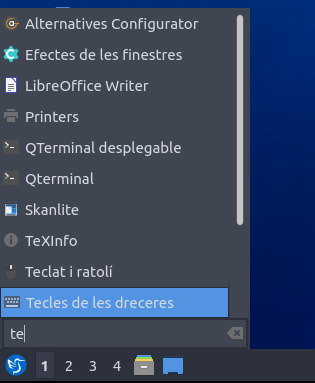
\includegraphics{png/Drecera0.png}
\caption{Figura1: Accedir a la configuració de dreceres}
\end{figure}

\subsubsection{Modificar una drecera
existent:}\label{modificar-una-drecera-existent}

Amb \emph{Control + T} obrim el QTerminal

\begin{figure}
\centering
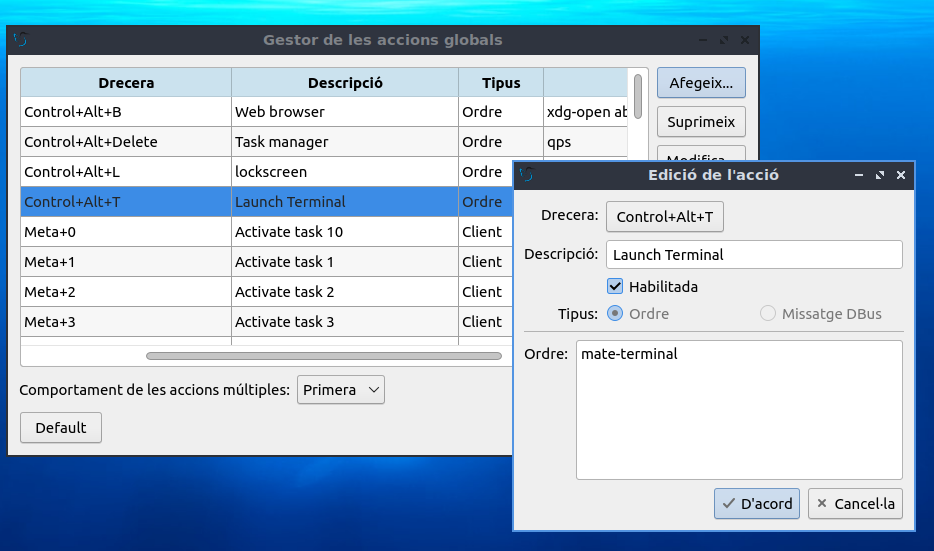
\includegraphics{png/Drecera1.png}
\caption{Figura2: Veiem quin programa crida}
\end{figure}

Canviem el nom del terminal\ldots{}

Ara obrirem el Mate-terminal que hem instal·lat.

\begin{figure}
\centering
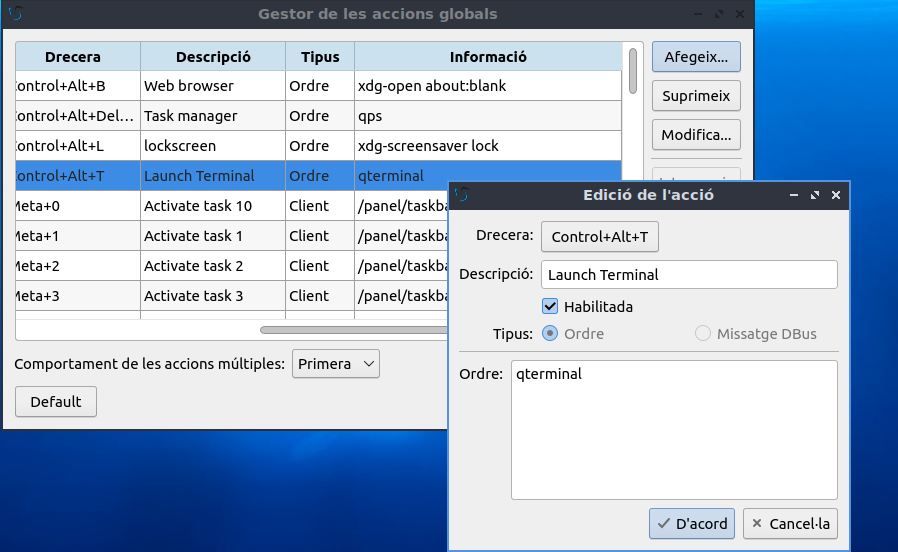
\includegraphics{png/Drecera2.png}
\caption{Figura3: Fem el canvi de programa}
\end{figure}

\subsubsection{Crear una drecera nova}\label{crear-una-drecera-nova}

Amb \emph{Control + E} obrirem el gestor de fitxers Caja (que devem
instal·lar)

\begin{figure}
\centering
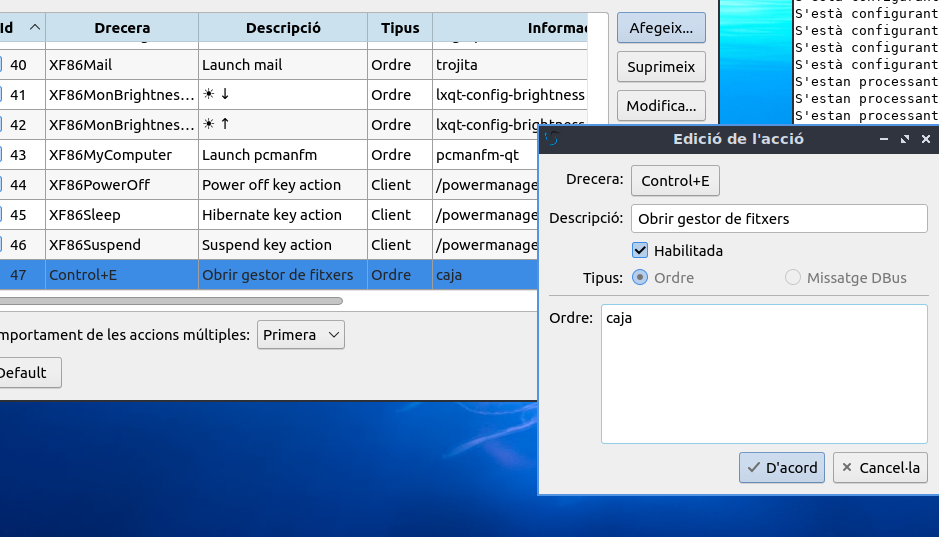
\includegraphics{png/Drecera3.png}
\caption{Figura4: Creem una nova drecera}
\end{figure}

\subsection{4.3 Aplicacions}\label{aplicacions}

\begin{itemize}
\tightlist
\item
  Navegador web: \textbf{Firefox}.
\item
  Suite ofimàtica: \textbf{LibreOffice}.
\item
  Reproductor multimèdia: \textbf{VLC}.
\end{itemize}

Habitualment entenem per aplicacions les que són gràfiques però no hem
d'oblidar que hi ha moltes eines que són aplicacions que s'executen en
mode CLI, encara que són software de sistemes per regla genearal. Les
hem anomenat al punt 1.2: apt, net-tools, nano, mdadm\ldots{}

La instal·lació ja hem vist que podem fer-la amb l'eina \emph{apt}. Més
avant ho repassarem i vorem altres formes.

\section{5 Conclusions}\label{conclusions}

Què podem dir ja de Linux o d'Ubuntu amb el que hem vist i el poc que
sabem de Windows o Android?

\textbf{Delimitació o capes:}

La primera cosa a destacar al món d'Ubuntu és la clara separació entre
nuclis, shell i GUI. Dins del GUI, veiem que també queda ben delimitat
el gestor de finestres, el gestors d'arxius dins del Escriptori.

\textbf{Diversitat i compatibilitat:}

La segona qüestió a destacar és la quantitat de Escriptoris, Gestors de
finestres, Gestors de fitxers i, fins i tot d'emuladors de terminals! i
la intercanviabilitat.

\emph{Compte que només estem veient una part del món Ubuntu. La galaxia
Linux és més gran i friqui encara!}

Tot açò junt a característiques com ser multiusuari (poder tindre
sessiona de terminal de distints usuaris al mateix temps) fa que siga
ideal per a una introducció al món del Sistema Operatius.

\end{document}
